\documentclass{beamer}
\usepackage{graphicx}
\usepackage{listing}
\usepackage[utf8]{inputenc}
\usetheme{Warsaw}

\beamertemplatenavigationsymbolsempty 

\title{Presentacion Teoria de Juegos}
\author{Silvio Vileriño}
\date{28 de julio de 2015}

\begin{document}

\begin{frame}
  \maketitle
\end{frame}

\begin{frame}
  \frametitle{Din\'amicas de competici\'on en escenarios de bienes comunes}
  \framesubtitle{Se presentan 3 modelos cl\'asicos}
  \begin{itemize}
    \setlength{\itemsep}{4pt}
    \item Vendedores de helados en la playa. \textbf{Hotelling, 1929}.
    \pause
    \item Dilema del prisionero. \textbf{Flood, Dresher, 1950}.
    \pause
    \item Tragedia de los comunes, \textbf{Harding, 1968}.
  \end{itemize}
\end{frame}

\begin{frame}
  \frametitle{Heladeros en la playa}
  \framesubtitle{Consideraciones}
  \begin{itemize}
    \setlength{\itemsep}{4pt}
    \item Tenemos una franja de playa con 80 personas tomando sol distribuidas uniformemente.    
    \pause
    \item Hay 2 heladeros, usted es uno de ellos.
    \pause
    \item Consideremos la franja de playa como una recta...
    \pause
    \item Podemos analizar esto desde varios puntos de vista...
  \end{itemize}
\end{frame}

\begin{frame}
  \frametitle{Heladeros en la playa}
  \framesubtitle{Consideraciones}

  \begin{itemize}
    \setlength{\itemsep}{4pt}
    \item Usted es el heladero posicionado en A, el otro heladero esta posicionado en B.
    \pause
    \item L, C, R son los turistas de la izquierda, centro y derecha respectivamente.
    \pause
    \item Usted vende helados a la region LAC.
    \pause
    \item El otro heladero vende helados a la region CBR.
    \pause
  \end{itemize}

  \begin{figure}[h!]
      \centering        
      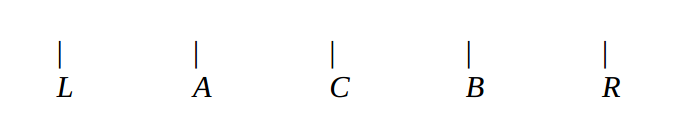
\includegraphics[scale=0.25]{fig/playa-posiciones.png}
      \caption{Posiciones en la porcion de playa}
  \end{figure}
\end{frame}

\begin{frame}
  \frametitle{Heladeros en la playa}
  \framesubtitle{Punto de vista de los turistas}

  \begin{itemize}
    \setlength{\itemsep}{4pt}
    \item Las mejores posiciones para los heladeros son en los cuartiles 0.25 y 0.75.
    \pause
    \item De esta manera, se minimiza la distancia promedio que debe caminar un turista para comprar helado a $\frac{1}{8}$ de playa.
    \pause
    \item Dadas estas condiciones, cada heladero espera vender un numero igual de helados, es decir, 40 helados.
  \end{itemize}
\end{frame}

\begin{frame}
  \frametitle{Heladeros en la playa}
  \framesubtitle{Punto de vista de los heladeros}

  \begin{itemize}
    \setlength{\itemsep}{4pt}
    \item Usted se da cuenta que desplazandose un poco a la derecha de su posicion original \textbf{(A)} puede aumentar su esperanza de ventas, capturando clientes a la derecha de la posicion central \textbf{(C)}, que ahora encuentran mas conveniente comprarle a usted porque esta mas cerca que el otro heladero.
    \pause
    \item El otro heladero, consciente de su desplazamiento y perdiendo clientes, toma la misma decision que usted, moviendose hacia la izquierda, aun mas distante de su posicion que usted.
    \pause
    \item Estos desplazamientos, \texttt{producen un aumento en la distancia media que los turistas deben caminar para comprar el helado}.
    \pause
    \item Este modo de pensar continua de parte de ambos vendedores, convergiendo en los dos vendedores en la posicion central, \texttt{con una misma tasa media de ventas}.
  \end{itemize}
\end{frame}

\begin{frame}
  \frametitle{Heladeros en la playa}
  \framesubtitle{Formalizando: Juego de suma cero}
  \begin{itemize}
    \setlength{\itemsep}{4pt}
    \item Consideremos las siguientes condiciones del problema
    \begin{itemize}
      \item Los vendedores comienzan en las posiciones A y B mencionadas al principio.
      \pause
      \item El total del mercado permanece constante(80 personas).
      \pause
      \item Conflicto directo, donde la ganancia de uno es la perdida del otro.
      \pause
      \item Los turistas no tienen problema con caminar demas ni cambiar de heladero.
      \pause
      \item Cada jugador(vendedor de helados) tiene 2 opciones: Moverse \textbf{(M)} o quedarse donde estaba originalmente (\textbf{NM}). 
    \end{itemize}
  \end{itemize}
\end{frame}

\begin{frame}
  \frametitle{Heladeros en la playa}
  \framesubtitle{Formalizando: Matrices de pago}
  \begin{itemize}
    \setlength{\itemsep}{4pt}
    \item Consideremos las siguientes matrices de pago para cada heladero
    \pause
    \item Si ninguno se mueve de A y B: Tienen mitad del mercado, distancia minima esperada para los turistas.   
    \pause
    \item Si ambos se mueven al centro: Tienen mitad del mercado, distancia esperada de los turistas aumenta.
    \pause
    \item Si uno se mueve y el otro no: El que queda en el centro tiene 50 turistas cautivos en su mercado, el otro 30.
    \pause    
  \end{itemize}

  \begin{figure}[h!]
      \centering        
      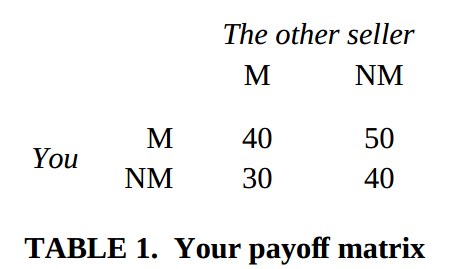
\includegraphics[scale=0.25]{fig/you-matrices-pago-playa.png}
      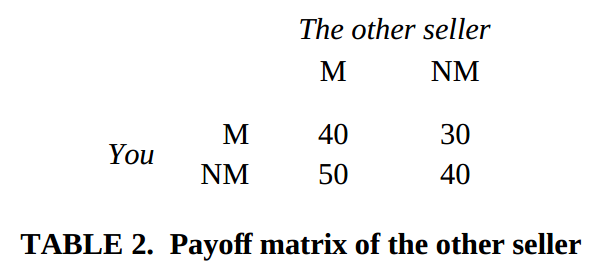
\includegraphics[scale=0.25]{fig/elotro-matrices-pago-playa.png}
      \caption{Matrices de pago}
  \end{figure}
\end{frame}

\begin{frame}
  \frametitle{Heladeros en la playa}
  \framesubtitle{Mejores Estrategias - Estrategias Dominadas}
  \begin{itemize}
    \setlength{\itemsep}{4pt}
    \item Observando las matrices de pagos de la slide anterior podemos concluir:
    \pause    
    \item Si el otro vendedor se mueve, me conviene moverme pare recuperar mercado perdido.
    \pause
    \item Si el otro vendedor no se mueve, me conviene moverme para capturar mas mercado.
    \pause
    \item Esto es simetrico para ambos jugadores.
    \pause
    \item En definitiva, la estrategia de moverse \textbf{domina} a la de no moverse.
  \end{itemize}
\end{frame}

\begin{frame}
  \frametitle{Heladeros en la playa}
  \framesubtitle{Estrategias desde el punto de vista de los turistas}
  \begin{itemize}
    \setlength{\itemsep}{4pt}
    \item Mas alla de que quedandose en los puntos A y B o ambos en el centro, la ganancia esperada de los heladeros no cambia...
    \pause
    \item La distancia esperada que debe caminar un turista al azar \textbf{se duplica de $\frac{1}{8}$ a $\frac{1}{4}$} si los heladeros se ponen ambos en el centro de la playa.
    \pause
    \item Tenemos entonces, un ejemplo en donde se observa que, a pesar de la creencia popular,
    \pause
    \item La competencia \textbf{No siempre} mejora el bienestar social. 
  \end{itemize}
\end{frame}

\begin{frame}
  \frametitle{Heladeros en la playa}
  \framesubtitle{Un escenario mas realista...}
  \begin{itemize}
    \setlength{\itemsep}{4pt}
    \item Consideremos ahora que los turistas consideran importante la distancia a un heladero
    \pause
    \item Los heladeros comienzan en A, B como antes, hay el mismo numero de turistas uniformemente distribuidos.
    \pause
    \item A medida que los heladeros se acercan al centro, el mercado se reduce...
    \pause
    \item Un turista deja de comprar helado si debe caminar mas de $\frac{1}{4}$ de porcion de playa.
    \pause
    \item Esto produce un cambio grande en las reglas del problema...Veamos...
  \end{itemize}
\end{frame}

\begin{frame}
  \frametitle{Heladeros en la playa II}
  \framesubtitle{Un escenario mas realista...}
  \begin{itemize}
    \setlength{\itemsep}{4pt}
    \item Si ningun heladero cambia de posicion, el mercado queda intacto(80 turistas)
    \pause
    \item Si solo uno se mueve al centro, el mercado se reduce a 60 turistas menos del lado del heladero que se mueve.
    \pause
    \item Si ambos se mueven al centro, el mercado se reduce a 40 turistas, dado que los turistas de los extremos dejaran de comprar helado por motivos de lejania.
    \pause
    \item Vemos que este es un juego de suma no nula. Formalicemos las matrices de pagos...
  \end{itemize}
\end{frame}

\begin{frame}
  \frametitle{Heladeros en la playa II}
  \framesubtitle{Modelando las matrices de pago...}
  \begin{itemize}
    \setlength{\itemsep}{2pt}
    \item Consideremos la siguiente matriz de pago para este problema y analicemos las estrategias asumiendo el rol del jugador de la izquierda en el par (x, y) de la matriz.
    \pause
    \item Si el otro vendedor se mueve, conviene no moverse.
    \pause    
    \item Si el otro vendedor no se mueve, conviene no moverse.
    \pause
    \item Mas aun, se tiene un incentivo(de 10 potenciales clientes nuevos) para convencer al otro vendedor de que no se mueva.
    \pause
    \item Simetricamente, el otro jugador tambien se quedara quieto en su posicion inicial.
    \pause
  \end{itemize}

  \begin{figure}[h!]
      \centering        
      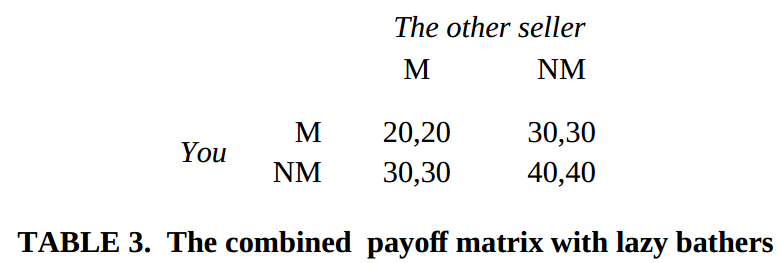
\includegraphics[scale=0.20]{fig/nonzero-matrices-pago-playa.png}
      \caption{Matriz de pago}
  \end{figure}
\end{frame}

\begin{frame}
  \frametitle{Heladeros en la playa II}
  \framesubtitle{Conclusiones...}
  \begin{itemize}
    \setlength{\itemsep}{4pt}
    \item Si ambos vendedores, en este modelo, comenzaran en el centro de la playa, les redituaria moverse hacia los percentiles 0.25 y 0.75.
    \pause
    \item En este caso, la competencia entre ambos vendedores beneficiaria a todos: Los vendedores abarcarian mas mercado y los turistas caminarian menos para obtener helado.
    \pause
    \item La afirmacion acerca del beneficio de la competencia para todos depende de los parametros particulares de la situacion: En este caso, la \texttt{demanda} de helado por parte de los turistas. 
  \end{itemize}
\end{frame}

\begin{frame}
  \frametitle{Heladeros en la playa III}
  \framesubtitle{Un modelo mas general...}
  \begin{itemize}
    \setlength{\itemsep}{4pt}
    \item Pensemos en el modelo anterior pero ahora definamos una proporcion $x \in \mathbb{R}$ como la distancia maxima que un turista esta dispuesto a recorrer para conseguir helado.
    \pause
    \item Podemos analizar la situacion en 2 casos.
    \pause
  \end{itemize}
    \begin{figure}[h!]
      \centering        
      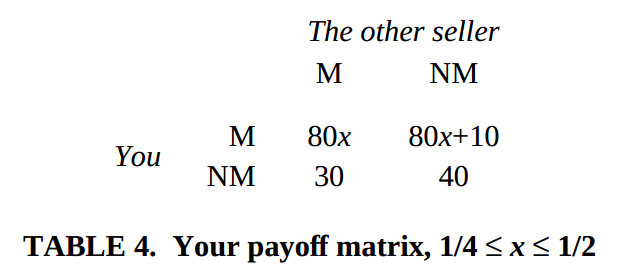
\includegraphics[scale=0.25]{fig/nonzero-matrices-pago-playa-14-12.png}
      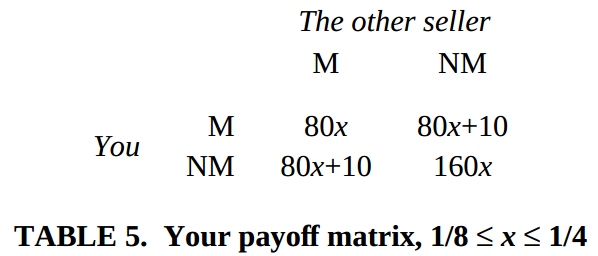
\includegraphics[scale=0.25]{fig/nonzero-matrices-pago-playa-18-14.png}
      \caption{Matriz de pago}
  \end{figure}
\end{frame}

\begin{frame}
  \frametitle{Heladeros en la playa III}
  \framesubtitle{Un modelo mas general...}
  \begin{itemize}
    \setlength{\itemsep}{4pt}
    \item Analizando las filas de las matrices de la slide anterior...
    \pause
    \item Si $ x \leq \frac{3}{8}$ la estrategia de no mover(sin importar que hace el otro jugador) paga mas que la estrategia de mover
    \pause    
    \item Para ver esto mas claramente, se muestran ploteos de la funcion de ganancia respecto a la distancia de tolerancia de los turistas a caminar para comprar helado.
  \end{itemize}
\end{frame}

\begin{frame}
  \frametitle{Heladeros en la playa III}
  \framesubtitle{Un modelo mas general...}

\begin{itemize}
    \setlength{\itemsep}{4pt}
    \item Funcion de ganancia respecto a la distancia.
    \pause
  \end{itemize}

  \begin{figure}[h!]
      \centering        
      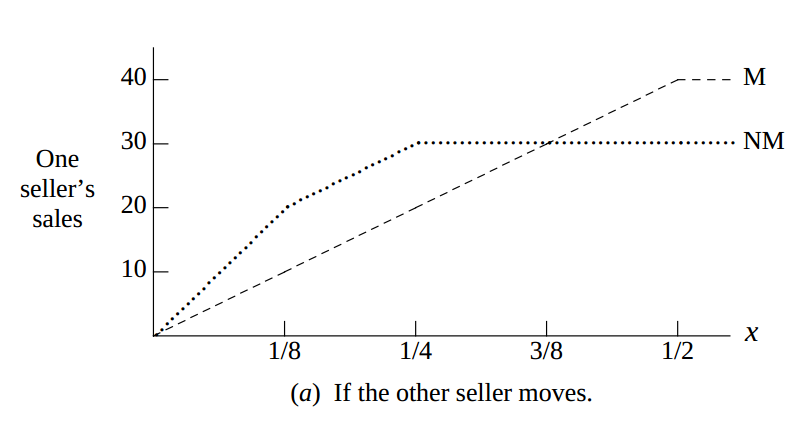
\includegraphics[scale=0.20]{fig/plot-pago-playa1.png}
      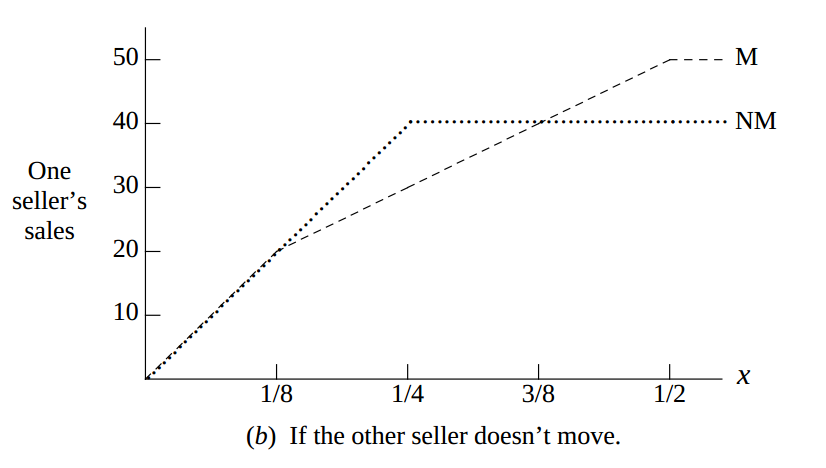
\includegraphics[scale=0.20]{fig/plot-pago-playa2.png}
  \end{figure}
\end{frame}


\begin{frame}
  \frametitle{Heladeros en la playa IV}
  \framesubtitle{Vendedores Ignorantes}
  \begin{itemize}
    \setlength{\itemsep}{4pt}
    \item El heladero A piensa que la distancia maxima que un turista va a caminar es $x > \frac{1}{2}$ de playa
    \pause
    \item El heladero B piensa que la distancia maxima que un turista va a caminar es $x = \frac{1}{4}$ de playa
    \pause    
    \item Si el heladero B piensa que A conoce la naturaleza vaga de los turistas al caminar por helado, va a esperar que el heladero A no se mueva, y tampoco va a moverse (con $x = \frac{1}{4}$ domina no moverse).
    \pause
    \item El heladero B, que ahora espera una ganancia de 40 turistas, ve que el heladero A se mueve, cayendo su ganancia a 30 turistas.
  \end{itemize}
\end{frame}

\begin{frame}
  \frametitle{Heladeros en la playa IV}
  \framesubtitle{Vendedores Ignorantes}
  \begin{itemize}
    \setlength{\itemsep}{4pt}
    \item Esto puede inducir(falsamente) al heladero B a pensar que los turistas en realidad no son vagos y el otro heladero esta vendiendo a 50, por lo tanto el tambien se mueve.
    \pause
    \item En este momento, donde ambos se han movido, han reducido a la mitad sus ganancias.
    \pause
    \item Como conclusion vemos que si ambos heladeros conocen el valor de $x$, van a elegir la mejor estrategia posible para ellos y los turistas.
  \end{itemize}
\end{frame}

\begin{frame}
  \frametitle{Modelo General}
  \framesubtitle{Generalizacion}
  \begin{itemize}
    \setlength{\itemsep}{4pt}
    \item Podemos pensar la franja de playa como cualquier caracteristica unidimiensional
    \pause
    \item Asimismo, podemos considerar la posicion de los vendedores como la magnitud de la caracteristica mencionada anteriormente.
    \pause 
    \item La distancia maxima que estaban dispuestos a caminar los turistas puede pensarse, como la tolerancia maxima al cambio de la caracteristica mencionada.
  \end{itemize}
\end{frame}

\begin{frame}
  \frametitle{Dilema del prisionero}
  \framesubtitle{Introduccion: Fur coat - Consideraciones}
  \begin{itemize}
    \setlength{\itemsep}{4pt}
    \item Existen 2 partes: vendedor y comprador
    \pause
    \item Cada uno esta satisfecho con lo que el otro le va a dar (producto y dinero).
    \pause 
    \item El intercambio debe ocurrir en un lugar secreto
    \pause
    \item Cada uno de los participantes dejara un bolso con la mercancia en un lugar predeterminado
    \pause
    \item Es claro que las 2 partes no volveran a verse ni a hacer negocios juntos
  \end{itemize}
\end{frame}

\begin{frame}
  \frametitle{Dilema del prisionero}
  \framesubtitle{Introduccion: Fur coat - Estrategias}
  \begin{itemize}
    \setlength{\itemsep}{4pt}
    \item Lo que ambas partes temen es que el otro les de un bolso vacio.
    \pause
    \item Claramente, si ambos cooperan y entregan los bolsos con la mercancia, ambos quedaran satisfechos.
    \pause
    \item Claramente tambien, si uno deja un bolso vacio y recibe la mercancia, estar\'a obteniendo algo por nada.
    \pause
    \item Esto nos lleva a una tentacion de dejar un bolso vacio.
    \pause
    \item De hecho,podemos razonar, con rigor aparente...
  \end{itemize}
\end{frame}

\begin{frame}
  \frametitle{Dilema del prisionero}
  \framesubtitle{Introduccion: Fur coat - Razonando no cooperativamente}
  \begin{itemize}
    \setlength{\itemsep}{4pt}
    \item Pongamosnos en el lugar de una de las partes...
    \pause
    \item Si el otro deja el bolso llena, me conviene dejar uno vacio, porque obtengo la mercancia gratis.
    \pause 
    \item Si el otro deja el bolso vacia, me conviene dejar uno vacio, porque no habre ganado nada, pero no pierdo mercancia tampoco.
    \pause
    \item Aparentemente, la mejor estrategia es dejar el bolso vacio.
    \pause
    \item El razonamiento del otro lado(otro participante) es identico.
  \end{itemize}
\end{frame}

\begin{frame}
    \frametitle{Dilema del prisionero}
  \framesubtitle{Introduccion: Fur coat - Razonando no cooperativamente}
  \begin{itemize}
    \setlength{\itemsep}{4pt}
    \item Entonces, con aparente logica, ambos dejan bolsos vacios.
    \pause
    \item Esto esta mal, porque ambos se vuelven a su casa con las manos vacias.
    \pause 
    \item Si hubieran confiado y cooperado les redituaria mas a ambos.
    \pause
    \item La logica previene la cooperacion? Esto es lo que presenta el \textbf{Dilema del prisionero}
  \end{itemize}
\end{frame}

\begin{frame}
    \frametitle{Dilema del prisionero}
  \framesubtitle{Idea original}
  \begin{itemize}
    \setlength{\itemsep}{4pt}
    \item Hay 2 prisioneros en salas de interrogacion separadas.
    \pause
    \item Cada uno tiene 2 opciones: Confesar o no un crimen.
    \pause 
    \item Existe evidencia circunstancial, pero las autoridades prefieren al menos una confesion.
    \pause
    \item Cada combinacion de estrategias entre ambos prisioneros tiene diferentes pagos...
    \pause
    \item Si ambos confiesan, ambos son condenados a un tiempo medio de prision.
    \pause
    \item Si ambos se quedan callados, ambos son condenados a un corto tiempo de prision.
    \pause
    \item Si uno confiesa y el otro no: El que confiesa es liberado, y el otro es condenado a un tiempo muy grande de prision.
  \end{itemize}
\end{frame}

\begin{frame}
    \frametitle{Dilema del prisionero}
  \framesubtitle{Matriz de pagos}
  \begin{itemize}
    \setlength{\itemsep}{4pt}
    \item Aunque se junten ambos prisioneros y discutan, llegando a la conclusion de que les conviene no confesar a ambos y beneficiarse mutuamente...
    \pause
    \item Pero individualmente, uno se da cuenta que existe la posibilidad de que el otro lo traicione...
    \pause 
    \item No solo dejando al otro prisionero en prision, sino tambien consiguiendo la libertad. 
    \pause
    \item De esta forma uno experimenta un gran incentivo para confesar, evitando asi la maxima condena de prision sin importar la decision de la contraparte.
    \pause
  \end{itemize}

  \begin{figure}[h!]
      \centering        
      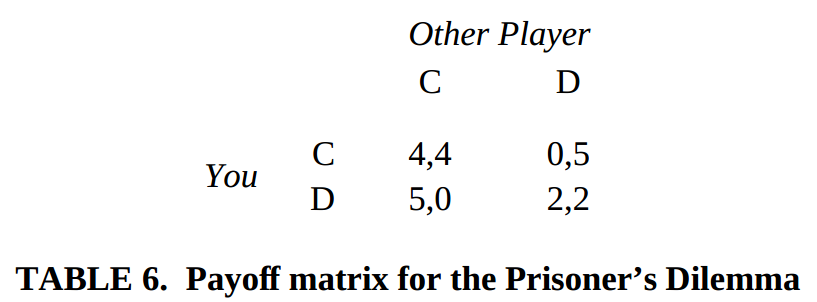
\includegraphics[scale=0.20]{fig/matrizpagos-prisionero.png}
  \end{figure}

\end{frame}

\begin{frame}
    \frametitle{Dilema del prisionero}
  \framesubtitle{Estrategias - Equilibrio de nash}
  \begin{itemize}
    \setlength{\itemsep}{4pt}
    \item Como los escenarios son simetricos para ambos prisioneros, ambos eligen confesar.
    \pause
    \item De nuevo, esto es triste porque si hubieran confiado entre ellos, hubieran tenido un mejor beneficio conjunto.
    \pause 
    \item Notemos que en este caso cada jugador conoce y adopta su mejor estrategia conociendo la estrategia de los demas.
    \pause
    \item Queda en un equilibrio de nash.
    \pause
    \item Notemos que en los equilibrios de nash no implican el mejor resultado conjunto para todos los participantes, sino solo el mejor resultado para cada uno considerado individualmente.
  \end{itemize}
\end{frame}

\begin{frame}
    \frametitle{Dilema del prisionero}
  \framesubtitle{Necesidad de \textbf{confianza} para obtener mejores resultados}
  \begin{itemize}
    \setlength{\itemsep}{4pt}
    \item Si ambos prisioneros pudieran convencerse mutuamente de cooperar, el resultado global seria mejor para ambos.
    \pause
    \item Este es un caso donde se necesita mejorar el \texttt{outcome} de la situacion por medio de \textbf{confianza}.
    \pause 
    \item En este ejemplo se observa que el comportamiento racional individual lleva a resultados inferiores para los individuos globalmente.
    \pause
    \item La competicion no traduce interes propio en el bien comun. 
  \end{itemize}
\end{frame}

\begin{frame}
  \frametitle{Dilema del prisionero}
  \framesubtitle{Algunos otros casos de la vida real...}
  \begin{itemize}
    \setlength{\itemsep}{4pt}
    \item En la economia de los paises, cada pais puede adoptar libre comercio o proteccionismo.
    \pause
    \item En conjunto estan mejor con libre comercio, pero basta con que uno no siga las reglas...
    \pause 
    \item En la politica, tenemos el ejemplo de la union sovietica y eeuu en la carrera armamentista.
    \pause
    \item Se puede trazar una analogia con el ejercicio del parcial, donde uno de los outcomes es la destruccion del planeta(menos infinito).
  \end{itemize}
\end{frame}

\end{document}